\rhead[\thepage]{\scriptsize{CAPÍTULO \thechapter}. \rightmark}
\lhead[CAPÍTULO \thechapter. \leftmark]{}
%======================================================================
\chapter{Cálculo infinitesimal}
\label{C1V}
\markboth{Cálculo}{Cálculo}
%======================================================================

Hay aplicaciones que piden ver cuanto cambia una cantidad o cuál es el área de cierta región. Si el intervalo de tiempo es amplio o si la región es cuadrada, el problema se puede resolver con la matemática ya vista. Ahora, si queremos tener una herramienta para calcular el área o saber el cambio instantáneo de una función cualquiera, debemos recurrir al cálculo. \\

En este capítulo recurriremos constantemente al dicho de Napoleón ``\textit{Divide y vencerás}'', esto es porque para los tópicos de límites, derivadas e integrales ocuparemos la noción de infinitesimal (significa muy pequeño). Al trabajar con partes pequeñas permite simplificar los cálculos de las pendientes en una función (derivadas) o el área bajo la curva (integrales).  

\section{Límites}
\label{C1V0}

En la sección (\ref{funrac0}) se habló de que era lo que ocurría con la función $f(x)$ cuando me acercaba por el lado positivo o por el lado negativo. Pero ¿Qué tan cerca me puedo acercar a un punto en una función? Esta respuesta la entrega los límites, que permite ver como se comporta la función en ese punto acercándose tanto como uno quiera.\\

Cuando una función está bien definida puedo saber su valor exacto de su imagen con cualquier valor del dominio, pero ocurre en ciertos casos que se busca el valor de la función justo en puntos que no está definida, por ejemplo las expresiones de fracciones. Veamos el siguiente caso:
\begin{eqnarray}
f(x)=\dfrac{x^{3}-1}{x-1}
\end{eqnarray} 
Puedo saber el valor de la función en cualquier punto menos cuando $x=1$, pero si me acerco lo suficiente puedo saber cuanto vale la función muy cerca del punto en el que se indetermina. Uno se puede acercar por dos lados, es decir, por los números positivos o los números negativos. Consiste en ir tomando valores del dominio cercanos al que se indetermina ($x\approx 1$) y ver la imagen que resulta.

\begin{table}[h!]
\begin{center}
 \begin{tabular}{|c|c|c|c|c|c|c|c|c|c|}
 \hline
 $x$&$0,75$&$0,9$&$0,99$&$0,999$&$1$&$1,001$&$1,01$&$1,1$&$1,25$\\
 \hline
 $f(x)$&$2,313$&$2,710$&$2,970$&$2,997$&?&$3,003$&$3,030$&$3,310$&$3,813$\\
 \hline
 \end{tabular}
 \caption{Tabla de valores para ver el valor de un límite.}
 \label{tablalim}
 \end{center}
\end{table}
Se ve en la tabla (\ref{tablalim}), que por ambos lados los números se acercan a un mismo valor. Entonces, se concluye que como tanto por la izquierda como por la derecha tiende al número $3$, el límite de la función cuando $x$ se acerca a $1$ es $3$. Su notación es
\begin{eqnarray*}
 \lim_{x\to 1 } f(x) &=&3\\
  \lim_{x\to 1 } \dfrac{x^{3}-1}{x-1} &=&3
\end{eqnarray*}
Nuevamente se debe repetir, yo me puede acercar cuanto yo quiera, es decir, puedo elegir un $x=0,99999...$ y estar muy cerca del valor en el punto que quiero, pero no es el valor de la función en ese punto ($x=1$).

\begin{mydef}
\textbf{Límite. }Sea $f(x)$ una función en un intervalo abierto que contiene al número $x_{0}$. El límite de la función $f(x)$ conforme $x$ se aproxima a $x_{0}$ es L, lo que se escribe como: 
\begin{eqnarray}
\lim_{x\rightarrow x_{0}}f(x)=L
\label{lim0}
\end{eqnarray}
Si la siguiente proposición es verdadera:\\
Dado cualquier $\epsilon>0$, no importa cuan pequeño sea, existe una $\delta>0$ tal que 
\begin{eqnarray*}
Si \hspace{4px} 0<|x-x_{0}|<\delta , \hspace{4px} entonces \hspace{4px} |f(x)-L|<\epsilon  
\end{eqnarray*}
\end{mydef}

 \begin{center}
\begin{figure}[h!]
\centering
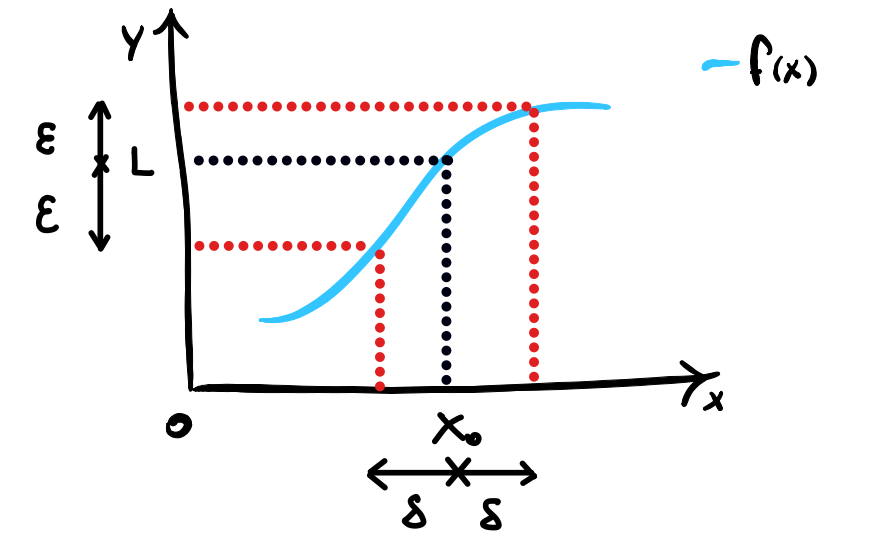
\includegraphics[scale=0.25]{limdef.png}
\caption[Gráfica de la definición de límite.]{Gráfica de la definición de límite. En el eje $x$ existe el parámetro $\delta$ y en el $y$ el parámetro $\epsilon$.} \label{limdef0}
\end{figure}
\end{center}
\newpage
En la ecuación (\ref{lim0}) de la definición se dice \textit{el límite de $f(x)$ cuando $x$ tiende a `a' es L}. Ahora, ya entendida la idea de lo que es el límite, veremos las diferentes reglas para calcularlos.

\noindent a) Límite de una función lineal. Si $m$ y $b$ son dos constantes cualesquiera, entonces \\
\begin{eqnarray}
\lim_{x\rightarrow a}(mx+b)=ma+b
\end{eqnarray}

\noindent b) Límite de una constante. Sea $c$ una constante, entonces para cualquier $a$ \\
\begin{eqnarray}
\lim_{x\rightarrow a}c=c
\end{eqnarray}

\noindent c) Límite de un polinomio de grado 1. \\
\begin{eqnarray}
\lim_{x\rightarrow a}x=a
\end{eqnarray}

\noindent d) Límite de una suma de límites. Si el límite de las funciones $f(x)$ y $g(x)$ son $L$ y $M$ respectivamente \\
\begin{eqnarray}
\lim_{x\rightarrow a}[f(x)\pm g(x)]=L\pm M
\end{eqnarray}
Esta propiedad es extensible para $n$ sumas o restas, pero aquí solo se considera el caso de dos límites.

\noindent e) Límite de una $n-$é$sima$ potencia de la función $f(x)$. Si la función $f(x)$ tiene como resultado del límite el número L, se cumple que \\
\begin{eqnarray}
\lim_{x\rightarrow a}f(x)^{n}=L^{n}
\end{eqnarray}

\noindent f) Límite de una expresión fraccional. Si las funciones $f(x)$ y $g(x)$ tienen como límite $L$ y $M$ respectivamente. Además, que $M\neq 0$ \\
\begin{eqnarray}
\lim_{x\rightarrow a}\dfrac{f(x)}{g(x)}=\dfrac{L}{M}
\end{eqnarray}

\noindent g) Límite de una raíz $n-$é$sima$. Si $n$ es un número entero positivo y el valor del límite de la función $f(x)$ es $L$ se cumple \\
\begin{eqnarray}
\lim_{x\rightarrow a}\sqrt[n]{f(x)}=\sqrt[n]{L}
\end{eqnarray}

\noindent h) Límite de una función fraccional particular. Si $a$ es cualquier número real distinto de cero se cumple \\
\begin{eqnarray}
\lim_{x\rightarrow a}\dfrac{1}{x}=\dfrac{1}{a}
\end{eqnarray}

\noindent i) Límite de una función fraccional cuando el límite tiende a infinito. 
\begin{eqnarray}
\lim_{x\rightarrow \pm\infty}\dfrac{1}{x}=0
\end{eqnarray}
\begin{myexample}
Calcular el límite de  las siguientes funciones:
\end{myexample}
\noindent\textit{i)}
\begin{eqnarray*}
\lim_{x\rightarrow 3}f(x)&=&\lim_{x\rightarrow 3}(x^{2}+7x-5)\\
&=&lim_{x\rightarrow 3}x^{2}+lim_{x\rightarrow 3}7x-lim_{x\rightarrow 3}5\\
&=&(3)^{2}+7\cdot (3)-5\\
&=&9+21-5\\
&=&25
\end{eqnarray*}
\noindent\textit{ii)}
\begin{eqnarray*}
\lim_{x\rightarrow 3}(3x+5)^{2}=14^{2}=196
\end{eqnarray*}

\noindent\textit{iii)}
\begin{eqnarray*}
\lim_{x\rightarrow\infty}\dfrac{\sqrt{4x^{2}+1}-2x}{x}&=&\dfrac{\sqrt{4x^{2}+1}-2x}{x} \cdot \dfrac{\sqrt{4x^{2}+1}+2x}{\sqrt{4x^{2}+1}+2x}\\
&=& \dfrac{(4x^{2}+1)-(2x)^{2}}{x(\sqrt{4x^{2}+1}+2x)}\\
&=&\dfrac{1}{2x}\\
\lim_{x\rightarrow\infty}\dfrac{\sqrt{4x^{2}+1}-2x}{x}&=&\lim_{x\rightarrow\infty}\dfrac{1}{2x}=0
\end{eqnarray*}

\subsection{Límites laterales}

Las expresiones que vimos anteriormente salvo un punto (singularidad) están definidas en todos los números reales, pero hay casos de funciones que su dominio está restringido y se quiere saber el límite. Ejemplo de esto son las raíces cuadradas.
\begin{eqnarray}
\lim_{x\rightarrow 2}=\sqrt{x-2}
\end{eqnarray}
El dominio de esta función no son todos los números reales, sino que para $x>2$. Entonces, al acercarse no lo podemos hacer por ambos lados, sino unicamente por los números positivos. Al calcular el límite se ve que es cero, pero hay que hacer la salvedad que es por la derecha, entonces se dice \textit{el límite de $f(x)$ por la derecha es cero}.

\begin{mydef}
\textbf{Límite por la derecha. }Sea una función $f(x)$ definida en cada número del intervalo abierto $]a,c[$. Entonces, el límite de $f(x)$, conforme $x$ tiende a $'a'$ por la derecha es L. Se denota por 
\begin{eqnarray*}
\lim_{x\rightarrow a^{+}}f(x)=L
\end{eqnarray*}
\end{mydef}

\begin{mydef}
\textbf{Límite por la izquierda. } Sea una función $f(x)$ definida en cada número del intervalo abierto $]a,d[$. Entonces, el límite de $f(x)$, conforme $x$ tiende a $'a'$ por la izquierda es L. Se denota por 
\begin{eqnarray*}
\lim_{x\rightarrow a^{-}}f(x)=L
\end{eqnarray*}
\end{mydef}

\begin{myexample}
La función signo (denotada sgn(x)) es la cual antes del cero es $-1$, en $x=0$ es $0$ y después del cero es $1$, por lo que se ve notoriamente si me acerco por las laterales el resultado de un límite va a ser distinto del otro. 
\begin{eqnarray*}
sgn(x)= \left\{\begin{array}{ll}
-1&, x< 0\\
0 &, x=0\\ 
1 &, x>0 \\
\end{array} \hspace{6px} \right.
\end{eqnarray*}
Calcule el límite de sgn(x). Primero el limite por la izquierda
\begin{eqnarray*}
\lim_{x\rightarrow 0^{-}}sgn(x)=-1
\end{eqnarray*}
Análogamente se calcula el límite por la derecha
\begin{eqnarray*}
\lim_{x\rightarrow 0^{+}}sgn(x)=1
\end{eqnarray*}
Se dice que la función no tiene límite. Además, una vez más sirve para recalcar que el valor de la función no tiene por qué ser el del límite en el punto, aunque este muy cerca. El valor de la función en $x=0$ es $0$ y los límites resultaron $1$ y $-1$ respectivamente. Si los límites laterales resultan el ser el mismo valor, entonces el límite existe. 
\end{myexample}

\begin{myexample}
Calcule el límite de la siguiente función por parte:\\

\[ f(x)= \left\{ \begin{array}{lcc} 
             4-x^{2} &   , si  & x\leq 1 \\
             \\ 2+x^{2} &  , si & x>1 \\
             \end{array}
   \right.\]\\
Calcule el $ \lim_{x\to 1^{+}}f(x)$ y $ \lim_{x\to 1^{-}}f(x)$.\\ %3\\

Según el caso del límite lateral reemplazamos en $f(x)$.

\begin{eqnarray*}
\lim_{x\to 1^{+}}(2+x^{2})&=& 2+(1)^{2}\\
&=& 3
\end{eqnarray*}
Análogamente para el otro caso
\begin{eqnarray*}
\lim_{x\to 1^{-}}(4-x^{2})&=& 4-(1)^{2}\\
&=& 3
\end{eqnarray*}
Como ambos límites laterales coinciden, entonces la función si tiene límite.
\end{myexample}

\section{Derivadas}

En la sección (\ref{cuociente0}) se dio las primeras pinceladas del problema que se resuelve en este capítulo. Ahí se planteó que se puede calcular  la pendiente de una curva tomando dos puntos cercanos, tan cercanos como uno desee. Esto tiene como consecuencia, que se termina calculando la pendiente de la función en dicho punto, es decir, el cambio que tiene en el eje $x$ y en el $y$. La diferencia de entre los puntos parte siendo la variable $h$ y en ese momento se escribió que $h$ se hace cero. Lo que haremos ahora es cambiar la notación para decir explícitamente que la pendiente es la razón de cambio en los ejes con la letra griega llamada \textit{Delta}.
\begin{mydef}
\textbf{Derivada de una función. } Si $f(x)$ es una función definida en un intervalo abierto que contiene a $c$ y además existe el límite
\begin{eqnarray}
\lim_{\Delta x\rightarrow 0 } &=&\dfrac{\Delta y}{\Delta x}\\
&=&  \lim_{\Delta x\rightarrow 0 }\dfrac{f(c+\Delta x)-f(c)}{\Delta x}
\label{limite0}
\end{eqnarray}
El resultado es una recta tangente a la gráfica de $f(x)$ en el punto (c,f(c)).
\end{mydef}

 \begin{center}
\begin{figure}[h!]
\centering
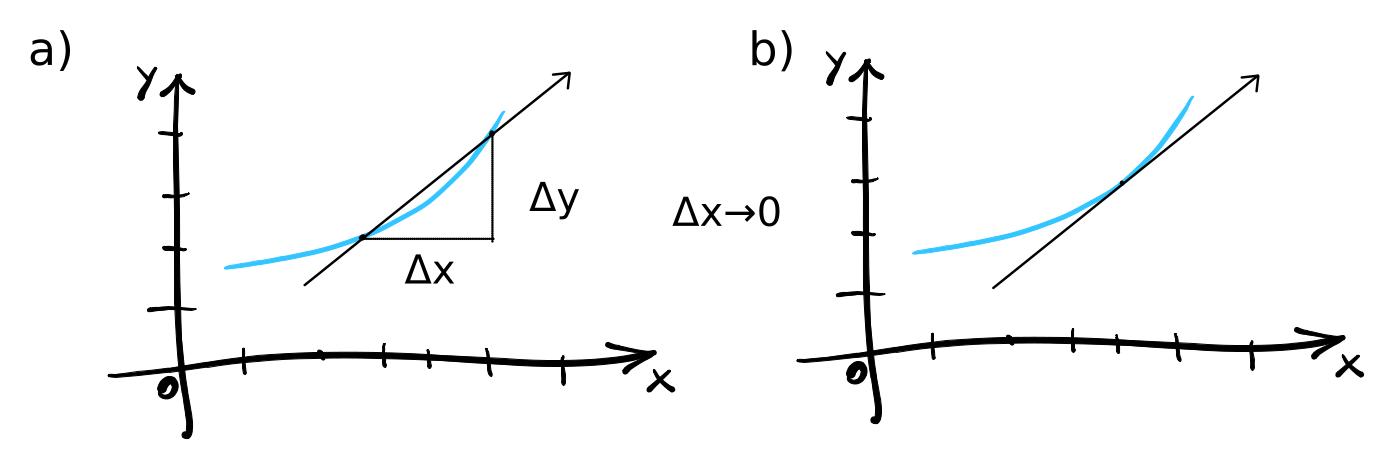
\includegraphics[scale=0.45]{der0.png}
\caption[Muestra gráfica de la definición de derivada para una variable.]{Muestra gráfica de la definición de derivada para una variable. a) $\Delta x$ representa cuanto cambia la función en el eje $x$ y $\Delta y$ muestra cuanto cambia la función en el eje $y$. b) Cuando se acercan demasiado los puntos resulta una recta tangente a la función, mostrando la pendiente de la función en ese punto.} \label{der0}
\end{figure}
\end{center}

La notación usual para la derivada de una función es $f'(x)$ o $df(x)/dx$, donde este último nos dice explícitamente con respecto a qué variable tenemos que derivar. Mencionar que si la función tiene derivadas en un punto es continua en ese punto,  es decir, no tiene un salto.

\subsection{Reglas de la derivación}
Resumiremos las principales reglas que tienen las funciones para derivarse. Es importante decir que no son las únicas y que aquí solo ocuparemos la regla, pero que cada una se puede comprobar con la expresión del límite de (\ref{limite0}).\\

\noindent a) Derivada de una constante:\\
\begin{eqnarray}
\dfrac{d}{dx}\left[c\right]&=&0
\end{eqnarray}

\noindent b) Derivada de una potencia:\\
\begin{eqnarray}
\dfrac{d}{dx}\left[x^{n}\right]&=&n\cdot x^{n-1}
\end{eqnarray}

\noindent c) Derivada de una función por una constante:\\
\begin{eqnarray}
\dfrac{d}{dx}\left[c\cdot f(x)\right]&=&c\cdot f'(x)
\end{eqnarray}

\noindent d) Derivada de una suma o resta:\\
\begin{eqnarray}
\dfrac{d}{dx}\left[f(x)\pm g(x)\right]&=& f'(x)\pm g'(x)
\end{eqnarray}

\noindent f) Derivada de una multiplicación:\\
\begin{eqnarray}
\dfrac{d}{dx}\left[f(x)\cdot g(x) \right]&=& f'(x)\cdot g(x)+g'(x)\cdot f(x)
\end{eqnarray}

\noindent g) Derivada del cuociente. Con $g(x)\neq 0$.\\
\begin{eqnarray}
\dfrac{d}{dx}\left[\dfrac{f(x)}{g(x)}\right]&=& \dfrac{f'(x)\cdot g(x)-f(x)\cdot g'(x)}{g(x)^{2}}
\end{eqnarray}

\noindent h) Regla de la cadena para una potencia. Considerar que $h(x)=f(g(x))$.\\
\begin{eqnarray}
\dfrac{d}{dx}\left[h(x)\right]&=& f'(g(x))\cdot g'(x)
\end{eqnarray}

\noindent i) Derivada de una función exponencial. Caso particular en que la base es el número $e$.\\

\begin{eqnarray}
\dfrac{d}{dx}\left[ e^{f(x)}\right]&=& e^{f(x)}\cdot f'(x)
\end{eqnarray}

\begin{myexample}
Utilizando las reglas de derivación que se mencionaron anteriormente, se resolverán los siguientes ejercicios
\end{myexample}
\noindent\textit{i)}
\begin{eqnarray*}
\dfrac{d}{dx}\left[5\right]&=&0
\end{eqnarray*}
\noindent\textit{ii)}
\begin{eqnarray*}
\dfrac{d}{dx}\left[x^{5}\right]&=&5\cdot x^{4}
\end{eqnarray*}
\noindent\textit{iii)}
\begin{eqnarray*}
\dfrac{d}{dx}\left[6\cdot (x^{2}+x^{7})\right]&=&6(2x+7x^{6})\\
&=& 6x(2+7x^{5})
\end{eqnarray*}
\noindent\textit{iv)}
\begin{eqnarray*}
\dfrac{d}{dx}\left[3x\cdot (x+2) \right]&=& 3(x+2)+3x\\
&=& 6x+6\\
&=& 6(x+1)\\
\end{eqnarray*}
\noindent\textit{v)}
\begin{eqnarray*}
\dfrac{d}{dx}\left[ \dfrac{x^{2}+2}{x^{3}-2}\right]&=& \dfrac{(2x)(x^{3}-2)-(x^{2}+2)(3x)}{(x^{3}-2)^{2}}\\
&=& \dfrac{(2x^{4}-4x)-(3x^{4}+6x^{2})}{(x^{3}-2)^{2}}\\
&=& \dfrac{(2x^{4}-4x)-3x^{4}-6x^{2}}{(x^{3}-2)^{2}}\\
&=& \dfrac{x(-x^{3}-4-6x)}{(x^{3}-2)^{2}}\\
&=& -\dfrac{x(x^{3}+4+6x)}{(x^{3}-2)^{2}}\\
\end{eqnarray*}
\noindent\textit{vi)}
\begin{eqnarray*}
\dfrac{d}{dx}\left[(x^{3}+5)^{2} \right]&=&2(x^{3}+5)3x^{2} \\
&=&6x^{2}(x^{3}+5) \\
&=&6x^{5}+30x^{2} \\
\end{eqnarray*}
\noindent\textit{vii)}
\begin{eqnarray*}
\dfrac{d}{dx}\left[e^{x^{2}}\right]&=&2xe^{x^{2}}
\end{eqnarray*}

\subsection{Derivada de orden superior}

La derivada es un operador, como la suma, que permite que se pueda aplicar cuantas veces sea necesario (siempre y cuando la función cumple ciertas condiciones que aquí no entraremos en detalles). Uno de los ejemplos más conocidos es en física. Si yo (el observador) sé la posición (coordenadas) de un objeto que se mueve, se puede derivar esa función una vez y saber su velocidad y si la derivo nuevamente sabré su aceleración.
\begin{eqnarray*}
f(t)&=& 2t^{2}=|\vec{r}|\\
\dfrac{df(t)}{dt}&=&2\cdot 2t=4t=|\vec{v}|\\
\dfrac{d^{2}f(t)}{dt^{2}}&=&4= |\vec{a}|\\
\end{eqnarray*} 
Esto se puede extender hasta $n$ casos, pero en este curso nos interesa hasta las derivadas de orden 2 (segunda derivada).

\begin{mydef}
\textbf{Derivadas de orden superior. } Sea de $f(x)$ una función derivable hasta el orden n. 
\begin{eqnarray}
f'(x)&=&\dfrac{df(x)}{dx}\\
f''(x)&=&\dfrac{d^{2}f(x)}{dx^{2}}\\
&\vdots  &\nonumber\\
f^{(n)}(x)&=&\dfrac{d^{n}f(x)}{dx^{n}}
\end{eqnarray}
\end{mydef}

\subsection{Extremos de una función}
Lo visto hasta el momento de derivadas nos permite ver aplicaciones para llegar a conclusiones de las funciones, tales como donde tiene un valor máximo, un valor mínimo, si es creciente o decreciente en cierto intervalo. 

\begin{mydef}
\textbf{Definición de extremos. } Sea un intervalo cualquiera $I$ que contiene al número $c$.
\begin{itemize}
	\item $f(c)$ es el mínimo de $f(x)$ en $I$ si $f(c)\leq f(x)$ para toda $x$ en $I$.\\
	 
	\item $f(c)$ es el máximo de $f(x)$ en $I$ si $f(c)\geq f(x)$ para toda $x$ en $I$. 
\end{itemize}
A los puntos extremos (o simplemente extremos) de una función se le llaman máximos y mínimos absolutos. 
\end{mydef}

Si la función está definida en un intervalo cerrado (esto es importante, que sea cerrado) y es continua en ese intervalo, entonces va a tener tanto un máximo como un mínimo en ese intervalo. Es importante mencionar que hasta el momento sabemos las que se necesita y cuando existen los puntos extremos, pero no se a visto como calcularlos.\\

Puede pasar que uno analiza funciones y presentan máximos y mínimos, pero pueden tener otros puntos más altos o más bajos que son los absolutos. Estos puntos se llaman máximos y mínimos relativos.

 \begin{center}
\begin{figure}[h!]
\centering
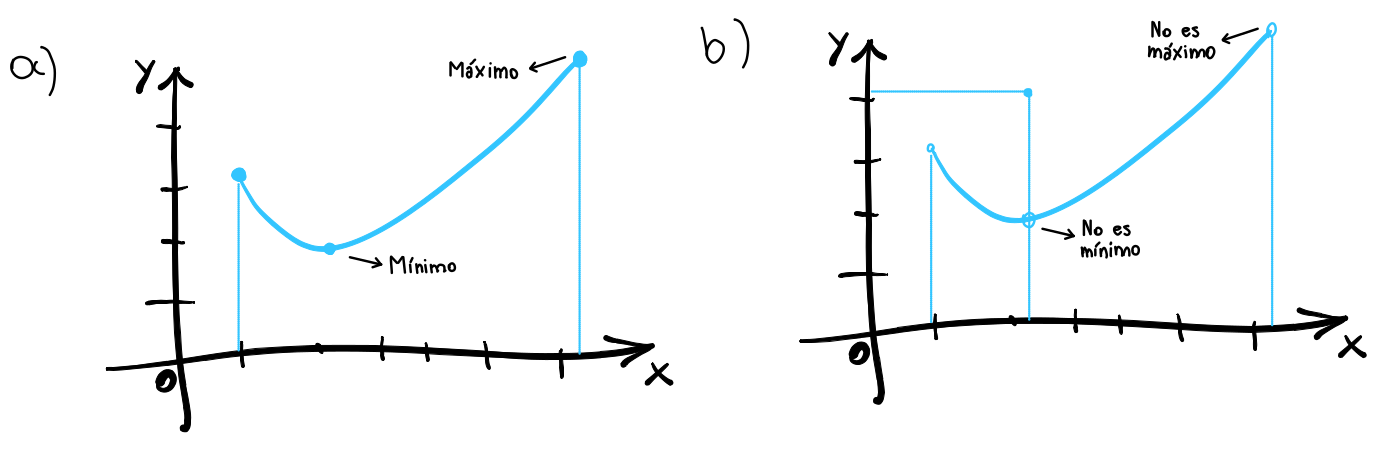
\includegraphics[scale=0.45]{der1.png}
\caption[Máximos y mínimos de una función.]{Máximos y mínimos de una función. a) Muestra una función definida en un intervalo cerrado (considera los extremos) por lo que la función tiene un máximo y un mínimo. b) La función está definida en un intervalo abierto y muestra una discontinuidad en el punto más bajo de la curva, por lo que no tiene mínimo ni máximo (No se puede derivar en ese punto).} \label{der1}
\end{figure}
\end{center}


\begin{mydef}
\textbf{Maxímos y mínimos relativos. } Sea f(x) definida en los números reales.

\begin{itemize}
\item  Si hay un intervalo abierto que contiene el punto $c$ en el cual $f(c)$ es el máximo, entonces $f(c)$ recibe el nombre de máximo relativo de $f(x)$.
\item Si hay un intervalo abierto que contiene el punto $c$ en el cual $f(c)$ es el mínimo, entonces $f(c)$ recibe el nombre de mínimo relativo de $f(x)$.
\end{itemize}
\end{mydef}

Ahora se muestra el procedimiento para encontrar los máximos y mínimos de una función definida en un intervalo cerrado $[a,b]$.\\
\begin{itemize}
	\item Se encuentran los puntos extremos de la función.\\
		\subitem Se calcula la derivada de primer orden.
		\subitem Se encuentran las raíces de la función derivada. $f'(x)=0$. Estos valores se consideran puntos críticos.
	\item Se evalúa $f(x)$ en cada punto crítico en el intervalo $]a,b[$.
	\item Se evalúa $f(x)$ en los puntos extremos del intervalo $[a,b]$. Reemplazar $f(x=a)$ y $f(x=b)$.
	\item Concluir que el valor más pequeño de los puntos encontrados es el mínimo y el más grande es el máximo de la función.
\end{itemize}

\begin{myexample}
Sea $f(x)=3x^{4}-4x^{3}$ definida en el intervalo cerrado $[-1,2]$. Calcular el o los máximos y mínimos relativos.
\begin{eqnarray*}
f(x)&=& 3x^{4}-4x^{3}\\
f'(x)&=& 12x^{3}-12x^{2}\\
\end{eqnarray*}
Ahora se iguala la deriva a cero.
\begin{eqnarray*}
f'(x)&=&0\\
12x^{3}-12x^{2}&=&0\\
12x^{2}(x-1)&=&0
\end{eqnarray*}
Los puntos críticos son $x=0$, $x=1$. Se deben evaluar estos puntos en la función $f(x)$.\\

\noindent $f(x=0)=0$.\\
\noindent $f(x=1)=-1$ Mínimo absoluto.\\
\noindent $f(x=-1)=7$\\
\noindent $f(x=2)=16$ Máximo absoluto.\\
\end{myexample}

\subsection{Función creciente y decreciente}
En la sección (\ref{funcrede}) se habló por primera vez de funciones crecientes y decrecientes, mostrando una leve introducción con su definición para poder clasificarlas. Ahora seguiremos hablando de ellas, pero mostraremos en que intervalo especifico muestra tal comportamiento. Estos intervalos están definidos por los puntos críticos de la función.\\
Con la operación de la derivada permite ahorrar camino y definir el comportamiento de la función con el resultado de la derivada en un intervalo dado. En el caso de una recta, si la derivada es positiva es una función creciente, es decir, su pendiente es positiva. Si es negativa, entonces es una función decreciente y si tiene derivada igual a cero es una función constante, este último caso es candidato a que tenga uno o más puntos críticos. Entonces, el procedimiento para encontrar el comportamiento de la función es el siguiente:

\begin{itemize}
	\item Calcular la derivada de primer orden de la función $f(x)$.
	\item Igualar la derivada a cero y encontrar las raíces de esa ecuación $f´(x)=0$.
	\item Separar los intervalos según los puntos críticos obtenidos.
	\item Tomar un $x$ del dominio según cada intervalo y reemplazarlo en la derivada de primer orden.
	\item Ver el valor de cada derivada y concluir si la función es creciente, decreciente o constante según resulte.
\end{itemize}

\begin{myexample}
Sea $f(x)=x^{3}-\dfrac{3x^{2}}{2}$. Determinar el comportamiento de $f(x)$.
\begin{eqnarray*}
f(x)&=& x^{3}-\dfrac{3x^{2}}{2}\\
f'(x)&=&3x(x-1)
\end{eqnarray*}
Las raíces de las derivadas son $x=0$ y $x=1$. Entonces, los intervalos son 3 y se resumen en la siguiente tabla:
\begin{table}[h!]
\begin{center}
		\begin{tabular}{|c|c|c|c|}
		\hline
		Intervalos & $-\infty <x<0$   & $0<x<1$&$1<x<\infty$ \\ 
		\hline
		 Signo de $f'(x)$&$x=-1$ &$x=1/2$ &$x=2$   \\
		 & $f'(x)=6>0$  & $f'(1/2)=-3/4<0$&$f'(2)=6$  \\
		\hline
		Criterio &Creciente&Decreciente& Creciente \\
		\hline
		\end{tabular}
		\caption{Comportamiento de los intervalos de la función.}
\end{center}
\end{table}
 \begin{center}
\begin{figure}[h!]
\centering
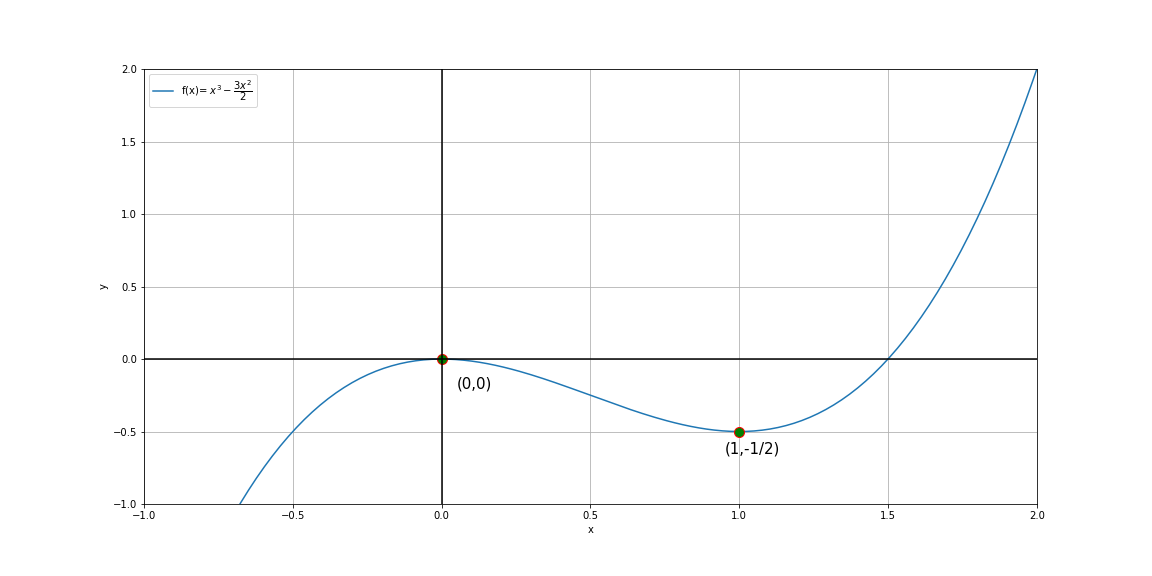
\includegraphics[scale=0.35]{ext0.png}
\caption{Gráfica de la función con los puntos críticos y sus cambios de comportamientos.} \label{ext0}
\end{figure}
\end{center}
\end{myexample}

Por lo visto, lo que ocurre en los puntos críticos es que el signo de la derivada cambia, ya sea de positivo a negativo  o viceversa. Entonces, si cambia de positivo a negativo es un máximo relativo y si cambia de negativo a positivo es un mínimo relativo o si tiene signos iguales antes y después del punto crítico no es ni máximo ni mínimo. Esto se le llama \textit{criterio de la primera derivada}.

\subsection{Concavidad y criterio de segunda derivada}

Con el criterio de la primera derivada se puede saber si la función crece o decrece en los intervalos, pero no sabemos como crece. El criterio de la segunda derivada viene a dar respuesta a ese problema, si crecen o decrecen con una curva hacia arriba o hacia abajo.

 \begin{center}
\begin{figure}[h!]
\centering
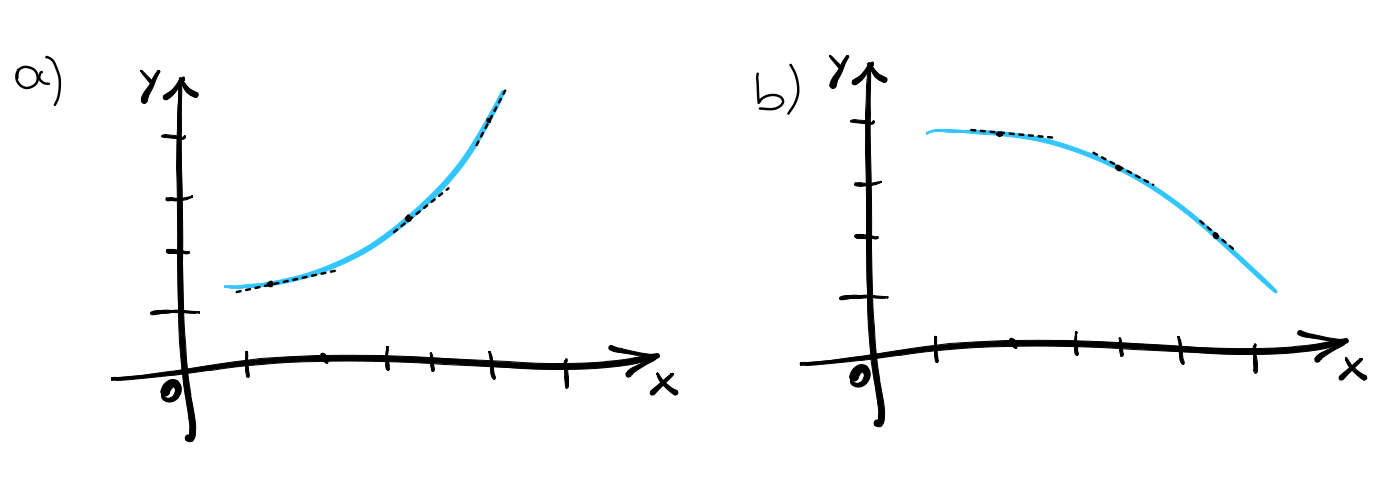
\includegraphics[scale=0.4]{con0.png}
\caption[Concavidad de las funciones.]{Concavidad de las funciones. a) Gráfica de una función con concavidad hacia arriba. b) Gráfica de una función con concavidad hacia abajo.} \label{con0}
\end{figure}
\end{center}

La función es cóncava hacia arriba si la derivada $f'(x)$ es creciente en el intervalo de observación. En el caso en que la derivada es decreciente, la función es cóncava hacia abajo.\\ 

\begin{mydef}
\textbf{Criterio de concavidad. } Sea $f(x)$ una función que permite la segunda derivada definida en un intervalo $I$.
\begin{itemize}
	\item Si $f''(x)>0$ para todo x en el intervalo $I$, entonces la gráfica de $f(x)$ es cóncava hacia arriba.
	\item Si $f''(x)<0$ para todo x en el intervalo $I$, entonces la gráfica de $f(x)$ es cóncava hacia abajo.
\end{itemize}
\end{mydef}

Ahora visto el criterio, el procedimiento para encontrar los rangos de concavidad es el siguiente: 
\begin{itemize}
	\item Calcular la derivada de primer y segundo orden de la función $f(x)$.
	\item Encontrar las raíces de la expresión de la segunda derivada. Dividir los intervalos en función de las raíces encontradas.
	\item Evaluar con un $x$ que se encuentre dentro de los intervalos y aplicar el criterio de concavidad.
\end{itemize}

\begin{myexample}
Sea $f(x)=\dfrac{x^{2}+1}{x^{2}-4}$. Encontrar la concavidad de sus intervalos.
\begin{eqnarray*}
f(x)&=&\dfrac{x^{2}+1}{x^{2}-4} \\
f'(x)&=&\dfrac{-10x}{(x^{2}-4)^{2}} \\
f''´(x)&=&\dfrac{10(3x^{2}+4)}{(x^{2}-4)^{3}} \\
\end{eqnarray*}
Los puntos críticos son $x=\pm 2$, por los que son 3 intervalos y se debe buscar tres concavidades.

\begin{table}[h!]
\begin{center}
		\begin{tabular}{|c|c|c|c|}
		\hline
		Intervalos & $-\infty <x<-2$   & $-2<x<2$&$2<x<\infty$ \\ 
		\hline
		 Signo de $f''(x)$&$x=-3$ &$x=0$ &$x=3$   \\
		 & $f''(x=-3)>0$  & $f''(x=0)<0$&$f''(3)>0$  \\
		\hline
		Criterio &C. hacia arriba &C. hacia abajo& C. hacia arriba \\
		\hline
		\end{tabular}
		\caption{Comportamiento de los intervalos de la función.}
\end{center}
\end{table}
 \begin{center}
\begin{figure}[h!]
\centering
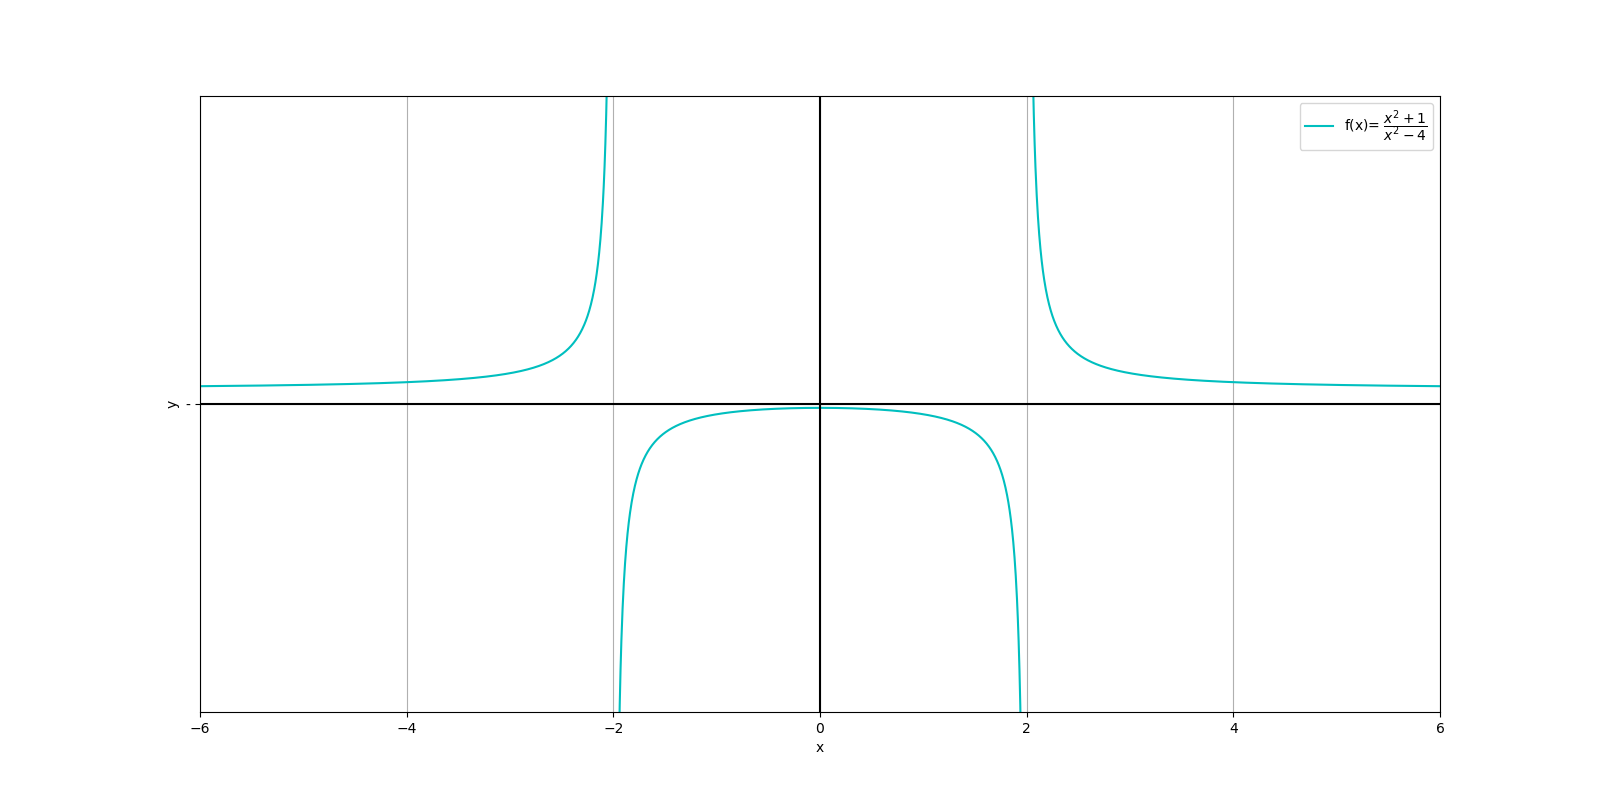
\includegraphics[scale=0.30]{ext1.png}
\caption{Gráfica de la función con las concavidades de cada intervalo.} \label{ext1}
\end{figure}
\end{center}
\end{myexample}

Los puntos que hacen cambiar la concavidad de la función $f(x)$ se les llama puntos de inflexión, es cuando la concavidad cambia de arriba a abajo o de abajo hacia arriba. Estos puntos no necesariamente son igual a un punto de un máximo o mínimo relativo.

\subsection{Criterio de la segunda derivada}
Para finalizar esta sección seguiremos exprimiendo la segunda derivada de una función. Cuando calculamos la derivada de primer orden y obtenemos los puntos críticos, para saber si es máximo o mínimo debemos calcular y ver los cambios de concavidad. La derivada de segundo orden permite evaluar estos puntos en la expresión y determinar para ahorrar cálculos

\begin{mydef}
\textbf{Criterio de la segunda derivada. } Sea $f(x)$ una función definida en los números reales y que acepta derivadas de primer y segundo orden. Además, si $f(x)$ tiene como punto crítico al número $c$. Entonces, basandonos en el criterio de la segunda derivada se puede concluir lo siguiente sobre el punto $c$
\begin{itemize}
 \item Si $f''(x)>0$, entonces $f(x)$ tiene un mínimo relativo en (c,f(c)).
 \item Si $f''(x)<0$, entonces $f(x)$ tiene un máximo relativo en (c,f(c)).
 \item Si $f''(x)=0$, el criterio falla y ahí hay que recurrir a la primera derivada y concavidad.
\end{itemize}
\end{mydef}

\begin{myexample}
Calcular los puntos críticos de $f(x)=-3x^{5}+5x^{3}$ y decir si son máximos o mínimos.
\begin{eqnarray*}
f(x)&=& -3x^{5}+5x^{3}\\
f'(x)&=&-15x^{4}+15x^{2}=15x^{2}(1-x^{2})\\
\end{eqnarray*}
Los puntos críticos son los valores $x=-1$, $x=0$ y $x=1$. Entonces, ahora se deben evaluar en la segunda derivada de la función. 
\begin{eqnarray*}
f''(x)&=& -60x^{3}+30x=30x(1-2x^{2})
\end{eqnarray*}

\begin{table}[h!]
\begin{center}
		\begin{tabular}{|c|c|c|c|}
		\hline
		Puntos & $x=-1$   & $x=0$&$x=1$ \\ 
		\hline
		 Signo de $f''(x)$&$x=-1$ &$x=0$ &$x=1$   \\
		 & $f''(x=-1)>0$  & $f''(x=0)<0$&$f''(1)<0$  \\
		\hline
		Criterio &Mínimo relativo &No entrega dato& Máximo relativo \\
		\hline
		\end{tabular}
		\caption{Criterio de la segunda derivada.}
\end{center}
\end{table}

 \begin{center}
\begin{figure}[h!]
\centering
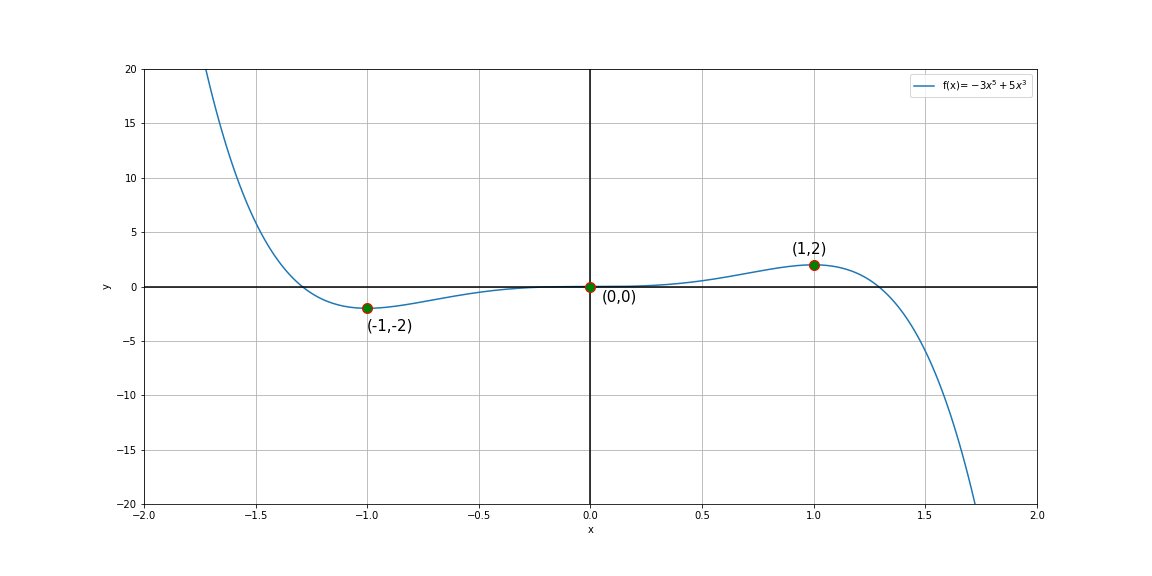
\includegraphics[scale=0.30]{ext2.png}
\caption{Gráfica de la función con los puntos críticos que demuestra el resultado del criterio de la segunda derivada.} \label{ext2}
\end{figure}
\end{center}

Se ve que la función tiene un punto máximo y un punto mínimo, pero que además hay un punto que el criterio no entrega información. 
\end{myexample}

\begin{myexample}
Se debe elegir un fármaco en base a que su tiempo de máxima concentración sea en el menor tiempo posible (tiempo en horas) ¿Cuál de los siguientes fármacos debo elegir?\\
\end{myexample}
\begin{center}
$C(t)_{1}=t-3t^{3}$ \\ $C(t)_{2}=48t-t^{3}$
\end{center}
\textit{Resp:}\\
\emph{Derivadas del primer fármaco}
\begin{eqnarray*}
C(t)_{1}&=&t-3t^{3}\\
C'(t)_{1}&=&1-9t^{2}\\
C''(t)_{1}&=&-18t\\
\end{eqnarray*}
De la derivada de primer orden obtenemos como punto crítico $t=\sqrt{1/9}$ de hora, se considera solo la raíz positiva ya que la unidad de medida es el tiempo. Ahora, lo evaluamos en la segunda derivada:\\
\begin{eqnarray*}
C''(t)_{1}&=&-18t\\
C''(1/3)_{1}&=&-18\left(\dfrac{1}{3}\right)=-6\\
\end{eqnarray*}

\emph{Derivadas del segundo fármaco}
\begin{eqnarray*}
C(t)_{2}&=&48t-t^{3}\\
C'(t)_{2}&=&48-3t^{2}\\
C''(t)_{2}&=&-6t\\
\end{eqnarray*}
De la primera derivada obtenemos el punto crítico $t=4$, nuevamente solo consideramos el de signo positivo. Ahora se evalúa en la segunda derivada.
\begin{eqnarray*}
C''(t)_{2}&=&-6t\\
C''(4)_{2}&=&-6(4)\\
C''(4)_{2}&=&-24\\
\end{eqnarray*}
Por el criterio de la segunda derivada ambos son máximos, pero el fármaco número 1 lo logra en menor tiempo y es el que se debe elegir.\\

 \begin{center}
\begin{figure}[h!]
\centering
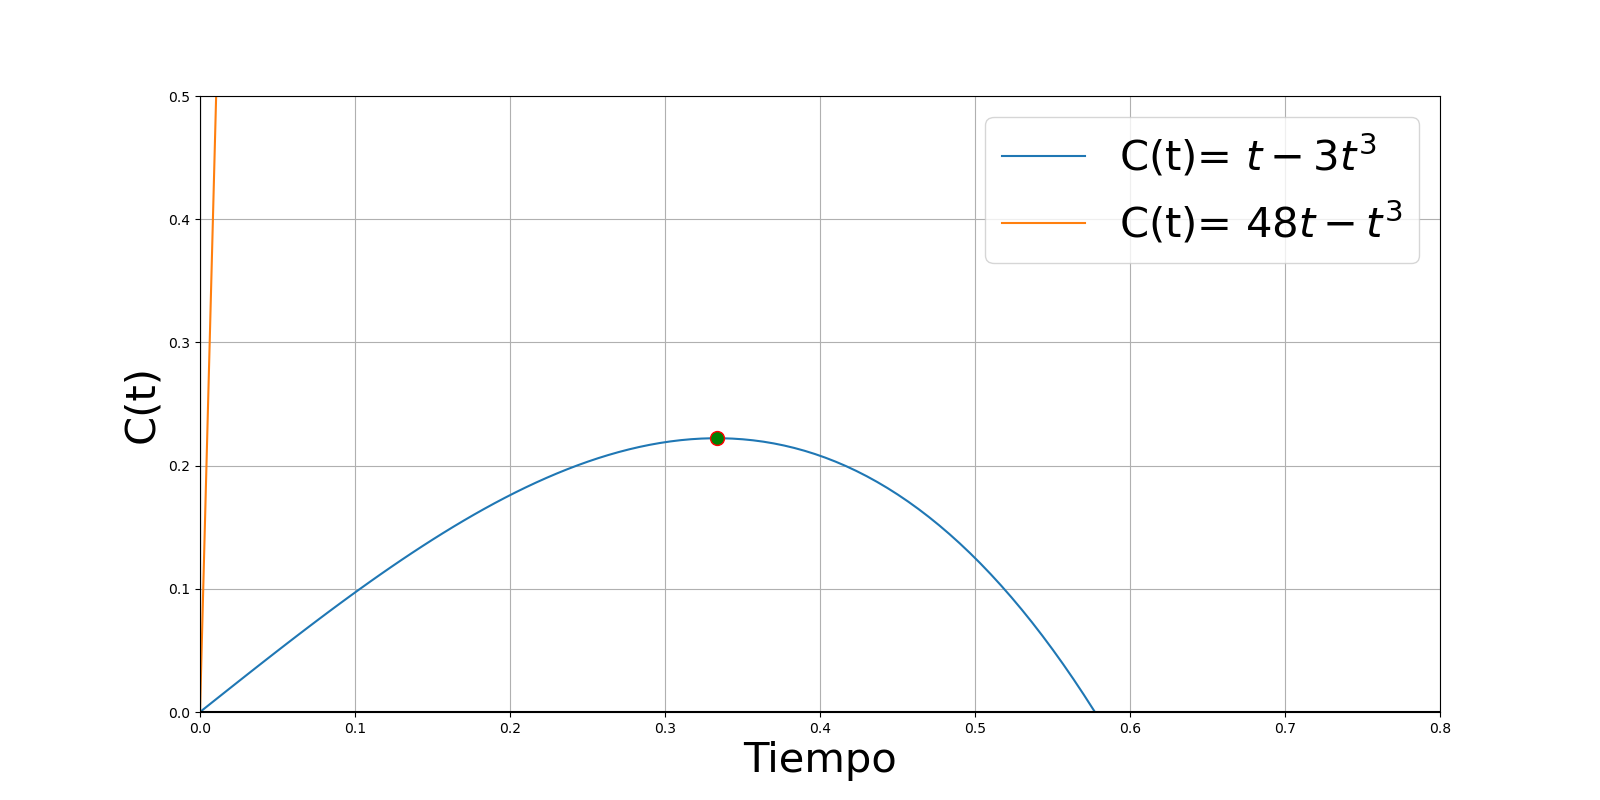
\includegraphics[scale=0.30]{farmacos.png}
\caption[Gráfico de las funciones de concentración de los fármacos.]{Gráfico de las funciones de concentración de los fármacos. El fármaco 1 (azul) llega mas rápido que el fármaco 2 (naranjo), aunque la concentración en el fármaco dos es mayor (no mostrada en la gráfica).} \label{farmacos}
\end{figure}
\end{center}

\begin{myexample}
 La presión arterial tiene un comportamiento periódico y se puede modelar (de forma muy sencilla) con un polinomio de la forma $ax^{3}-bx^{2}+cx$, donde $a$ es la presión diastólica media (PD)\footnote{Es la presión sobre las arterias cuando el corazón se relaja entre latidos, por lo tanto es el menor valor al momento de medir la presión arterial}, $b$ es la presión sistólica media (PS)\footnote{Es la presión ejercida cuando el corazón bombea la sangre, por lo tanto es el valor mas grande al momento de medir la presión} y $c$ es la edad de la persona (E). Encuentre el máximo (El peak sistólico), el mínimo (El peak diastólico) y el punto de inflexión ($f''(x)=0$) para el caso de una niña de 10 años con PD=120 y PS=80.\\
\end{myexample}
\textit{Resp:}\\
Derivadas de la función:
\begin{eqnarray*}
f(x)&=&ax^{3}-bx^{2}+cx\\
f(x)&=&120x^{3}-80x^{2}+10x\\
f'(x)&=&360x^{2}-160x+10\\
f''(x)&=&720x-160\\
\end{eqnarray*}
De la derivada de primer orden se obtienen de puntos críticos $x=\dfrac{2}{9}\pm\dfrac{\sqrt{7}}{18}$
\begin{eqnarray*}
f''\left(\dfrac{2}{9}+\dfrac{\sqrt{7}}{18}\right)&=& 720\left(\dfrac{2}{9}+\dfrac{\sqrt{7}}{18}\right)-160 \\
&=& 40\sqrt{7}>0\\
\end{eqnarray*}
Análogamente con el otro punto
\begin{eqnarray*}
f''\left(\dfrac{2}{9}-\dfrac{\sqrt{7}}{18}\right)&=& 720\left(\dfrac{2}{9}-\dfrac{\sqrt{7}}{18}\right)-160 \\
&=&-40\sqrt{7}<0\\
\end{eqnarray*}
$x=\dfrac{2}{9}+\dfrac{\sqrt{7}}{18}$ es un mínimo y $x=\dfrac{2}{9}-\dfrac{\sqrt{7}}{18}$ es máximo. Finalmente, se calcula en punto que cambia la concavidad, es decir, cuando la segunda derivada es cero.
\begin{eqnarray*}
f''(x)&=&720x-160=0\\
x&=&\dfrac{160}{720}\\
x&=&\dfrac{2}{9}\\
\end{eqnarray*}

 \begin{center}
\begin{figure}[h!]
\centering
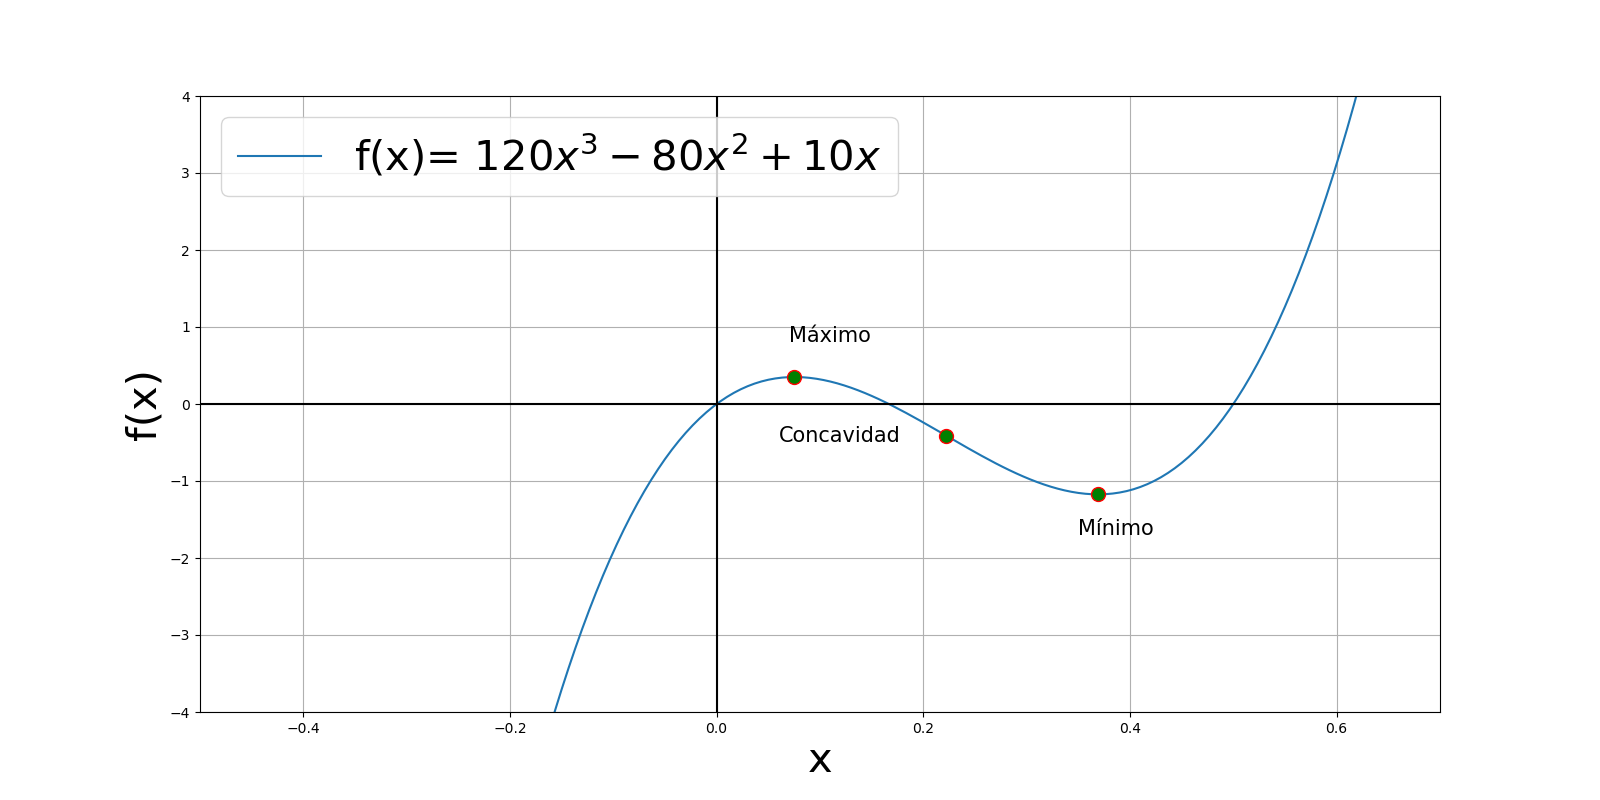
\includegraphics[scale=0.30]{latidos.png}
\caption[Gráfico del modelo polinómico del periodo arterial.]{Gráfico del modelo polinómico (Bien simple) del periodo arterial. Los puntos verdes representan el máximo (Peak sistólico), el mínimo (Peak diastólico) y el cambio de concavidad.} \label{farmacos}
\end{figure}
\end{center}
\section{Integrales}

Con esta sección damos por finalizado el capítulo de cálculo, donde por tercera vez recurriremos a lo infinitesimal.\\

Hay instancias en que se busca calcular el área de alguna figura y esto no ha sido problema hasta el momento, porque las fórmulas de esas figuras las sabemos (el área de cuadrados, triángulos, trapecios, etc.), pero si se complica un poco la situación y la figura es más rara de lo que conocemos quedamos de brazos cruzados. Entonces, varios matemáticos como Isaac Newton\footnote{Isaac Newton, Físico y matemático inglés. 1642-1727.} y Gottfried Leibniz\footnote{Gottfried Wilhelm Leibniz, Matemático y teólogo alemán. 1649-1716. Introdujo el símbolo de la integral, que representa una S alargada, por la suma de las áreas.} sementaron las bases del cálculo, entre ellos se pensó en dividir en partes pequeñas, muy pequeñas, para resolver este problema. No fue hasta Bernhard Riemann\footnote{
Bernhard Riemann, Matemático alemán. 1826-1866.} que se formalizó la integración utilizando límites. La integral es el área bajo  la curva que se dividió en rectángulos muy pequeños para luego sumar el área de todos ellos. Resulta que esa área se puede aproximar y queda la integral de la función. La representación de la figura (\ref{int0}) muestra como es una buena aproximación sumar los rectángulos de ancho $dx$ y de alto $f(x)$. 

\begin{center}
\begin{figure}[h!]
\centering
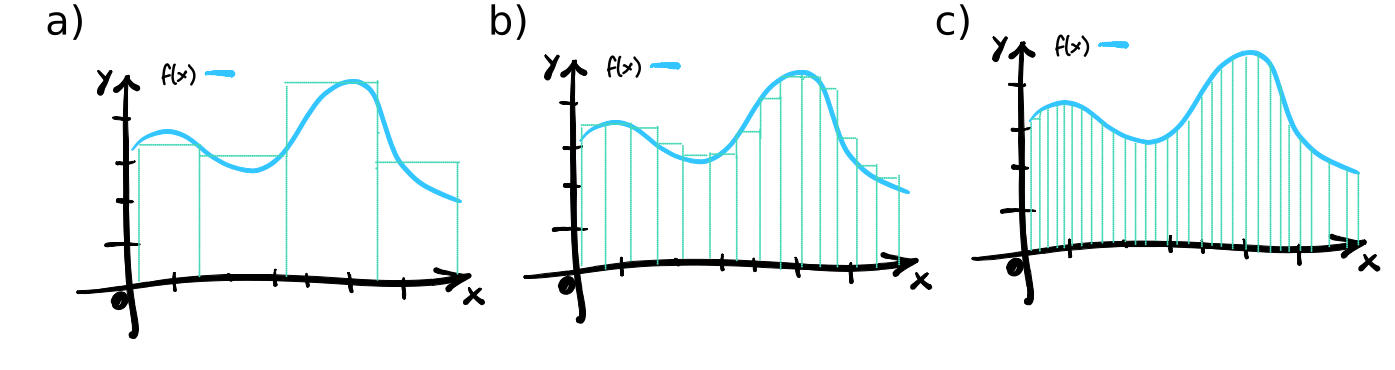
\includegraphics[scale=0.45]{int0.png}
\caption[Representación de la integral.]{Representación gráfica de la integral. Desde la figura a) a la c) se va viendo como el rectángulo se hace más pequeño para que el área bajo la curva sea igual al área de la función.} \label{int0}
\end{figure}
\end{center}

Así como el función logarítmica y la función exponencial son funciones inversas, las derivadas y las integrales lo son. Cuando uno tiene una expresión $f(x)$ y se aplica una integración obtiene una expresión llamada la antiderivada y que si uno la deriva vuelve a la misma expresión inicial $f(x)$.


\newpage
\begin{mydef}
\textbf{Antiderivada. } Sea F(x) y F'(x) su derivada que podemos llamar f(x), es decir, $F'(x)=f(x)$. Se dice que $F(x)$ es la antiderivada de $f(x)$.
\end{mydef}

En el gráfico (c) de la figura (\ref{int0}) se ven varios rectángulos muy pequeños, entonces al momento de calcular el área se debe multiplicar la base que llamaremos $dx$ por el alto, que es el valor de la función $f(x)$. El área de cada rectángulo es $f(x)\cdot dx$ y si los sumamos, aparece la expresión de la integral 
\begin{eqnarray}
y=\int f(x)dx= F(x)+C
\label{integral}
\end{eqnarray}
La ecuación (\ref{integral}) está confirmando que se suma el área de los rectángulos (símbolo de la integral). Además, como resultado entrega la antiderivada más una constante arbitraria.\\
La constante muestra que hay varias soluciones para una misma integral, además se ve la relación que hay entre las derivadas e integrales como operaciones inversas.
\begin{myexample}
Derivar e integrar las siguientes expresiones:
\end{myexample}
\begin{eqnarray*}
f(x)=50x^{2}+x+20 \hspace{15px} &y& \hspace{15px} g(x)=50x^{2}+x+40\\
f'(x)=\dfrac{df(x)}{dx}=100x+1 &y& g'(x)=\dfrac{dg(x)}{dx}=100x+1\\
\int f'(x)dx =\int (100x+1)dx &y& \int g'(x)dx = \int (100x+1)dx \\
50x^{2}+x+C &y& 50x^{2}+x+C
\label{constC}
\end{eqnarray*}
Para $f(x)$ la constante vale 20, mientras que para $g(x)$ vale 40. Entonces, de momento se obtiene una \textit{familia de soluciones} cuando se integra, y se llama solución general. 
\subsection{Reglas de integración}

\noindent a) Derivada de una integral: \\
\begin{eqnarray}
\dfrac{d}{dx}\left[ \int  f(x)dx \right]&=& f(x)
\end{eqnarray}

\noindent b) Integral del cero: \\
\begin{eqnarray}
\int 0dx &=& C
\end{eqnarray}

\noindent c) Integral de una constante:\\
\begin{eqnarray}
 \int kdx &=& kx + C
\end{eqnarray}

\noindent d) Integral multiplicada por una constante:\\
\begin{eqnarray}
 \int kf(x)dx &=&  k\int f(x)dx 
\end{eqnarray}

\noindent e) Integral de una suma o resta:\\
\begin{eqnarray}
 \int \left[f(x)\pm g(x) \right]dx &=&\int f(x)dx \pm \int g(x)dx 
\end{eqnarray}

\noindent e) Integral de una potencia:\\
\begin{eqnarray}
 \int x^{n}dx &=&\dfrac{x^{n+1}}{n+1} +C
\end{eqnarray}
Donde $n$ es número real.

\noindent f) Integral de una función exponencial. Caso particular donde la base es el número $e$ y el exponente es un exponente de grado $1$.\\
\begin{eqnarray}
 \int e^{x}dx &=&e^{x} +C
\end{eqnarray}

\noindent g) Integral de una función exponencial. Caso particular en que el coeficiente $n$, que acompaña a la variable del exponente es $\neq 1$.\\

\begin{eqnarray}
 \int e^{nx}dx &=&\dfrac{e^{nx}}{n} +C
\end{eqnarray}

\noindent h) Integrales de las principales funciones trigonometricas
\begin{eqnarray}
\int cos(x)dx= sen(x)+ C ; \hspace{6px} \int sen(x)dx= -cos(x)+C ; \\
 \int sec(x)^{2}dx= tan(x)+C; \hspace{6px} \int sec(x)tan(x)dx= sec(x)+ C \\
 \int csc(x)^{2}dx= -ctan(x)+C ; \hspace{6px}  \int csc(x)ctan(x)dx= -csc(x)+C
\end{eqnarray}
 
\begin{myexample}
En base a las reglas mostradas anteriormente se resolverán las siguientes integrales:
\end{myexample}
\noindent\textit{i)}
\begin{eqnarray*}
\dfrac{d}{dx}\left[ \int  (2x^{2})dx \right]&=& 2x^{2}
\end{eqnarray*} 
 \noindent\textit{ii)}
\begin{eqnarray*}
 \int 5dx &=& 5x + C
\end{eqnarray*} 
\noindent\textit{iii)}
\begin{eqnarray*}
 \int \dfrac{1}{\sqrt{2}}x^{2} dx &=&   \dfrac{1}{\sqrt{2}}\int x^{2}dx = \dfrac{1}{\sqrt{2}} \left[\dfrac{x^{3}}{3}+C \right]= \dfrac{x^{3}}{3\sqrt{2}} +C
\end{eqnarray*}
Se debe notar que $C$ es una constante y que si se multiplica por un factor, seguirá siendo una constante. Entonces, se puede seguir escribiendo como $C$ o cambiar de letra la constante y no se pierde generalidad.\\ 
\noindent\textit{iv)}
\begin{eqnarray*}
 \int (6x^{3}+7x^{2})dx = \int 6x^{3}dx+\int 7x^{2}dx &=& 6\left[\dfrac{x^{4}}{4}+C \right]+7\left[\dfrac{x^{3}}{3}+D\right]\\
&=& \dfrac{6x^{4}}{4}+C+\dfrac{7x^{3}}{3}+D \\
&=& \dfrac{6x^{4}}{4}+\dfrac{7x^{3}}{3}+E, \hspace{25px} C+D=E
\end{eqnarray*} 
\noindent\textit{v)}
\begin{eqnarray*}
 \int 5x^{3}dx &=& \dfrac{5x^{4}}{4} + C
\end{eqnarray*} 
\noindent\textit{vi)}
\begin{eqnarray*}
 \int (4x^{2}+3x)dx &=&  \int 4x^{2}dx+\int 3xdx\\
 &=&  \dfrac{4x^{3}}{3}+\dfrac{3x^{2}}{2}+C \\
\end{eqnarray*} 
\noindent\textit{vii)}
\begin{eqnarray*}
 \int e^{x}dx &=&  e^{x} + C
\end{eqnarray*} 
\noindent\textit{viii)}
\begin{eqnarray*}
 \int e^{3x}dx &=&  \dfrac{e^{3x}}{3} + C
\end{eqnarray*} 

En el ejemplo (\ref{constC}) se ve y se menciona que para funciones distintas, $f(x)$ y $g(x)$, se encuentran la misma antiderivada. La diferencia la marca la constante $C$, que tiene valores distintos. Entonces, se encuentran funciones que están desplazas por una cantidad $C$. Para encontrar el valor de esta constante se necesita información adicional, a la cual se llaman condiones iniciales. Consta de saber el valor de la función para un determinado valor de $x$, y luego despejar la constante C. 
 \begin{myexample}
 Sea $f(x)=x^{2}+5x$, encuentre la solución general de la integral de $f(x)$
 \label{ejemploConst}
 \end{myexample}
 \begin{eqnarray*}
 \int (x^{2}+5x)dx= \dfrac{x^{3}}{3}+ \dfrac{5x^{2}}{2}+C
 \end{eqnarray*}

\begin{figure}
\centering
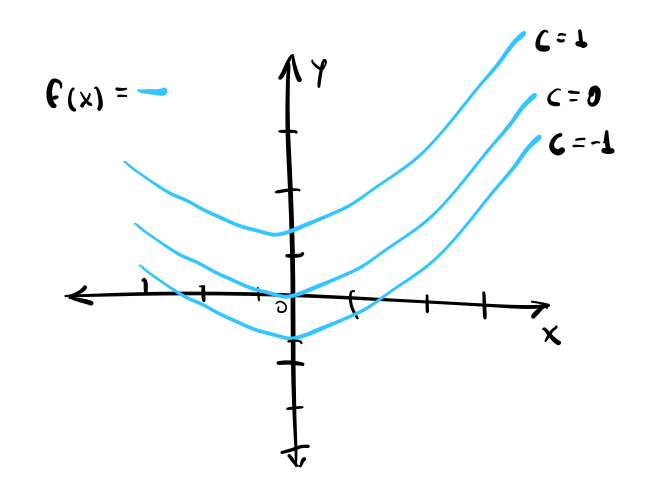
\includegraphics[scale=0.3]{ConstaC.png}
\caption{Casos de la función $f(x)$ del ejemplo (\ref{ejemploConst}) para tres valores distintos de la constante C.}
\end{figure} 
 
 \begin{myexample}
El decaimiento de un medicamento a través del tiempo (la razón de cambio) está dado por la expresión $df(x)/dx=e^{-\kappa t}$, donde la cosntante de decrecimiento está dado $\kappa =2$. Además se sabe que el tiempo inicial ($t=0$) hay 100ml del medicamento. Integrar la derivada y econtrar la constante $C$. 
\end{myexample}
\begin{eqnarray*}
\int \dfrac{df(x)}{x}&=& e^{-\kappa t} +C \\
&=& e^{-2 t}+C \\
\end{eqnarray*}
Se agrega la condición inicial para el tiempo inicial ($t=0$)
\begin{eqnarray*}
e^{-2 \cdot 0}+C &=& 100\\
1+C &=& 100 \\
C= 99
\end{eqnarray*} 
\subsection{Integrales definidas y teorema fundamental del cálculo}

En la sección anterior se vieron las integrales indefinidas y sus reglas de integración, pero usualmente uno necesita agregar limites para obtener un resultado con sentido en los problemas (tiempo, metros, litros, etc), lo que permite definir un rango de integración y en ese caso, la integral pasa llamarse \textit{integral definida}. Los límites entre los cuales quiero integrar se llaman límites de integración.

\begin{mydef}
\textbf{Teorema fundamental del cálculo. } Si una función $f(x)$ es continua en el intervalo cerrado $[a,b]$ y F es la antiderivada de la función f(x) en el intervalo $[a,b]$, entonces se cumple lo siguiente:
\begin{eqnarray}
\int_{a}^{b}f(x)dx=F(b)-F(a) \hspace{20px} o \hspace{20px} -\int_{b}^{a}f(x)dx=F(a)-F(b)
\end{eqnarray}
Se puede resumir en que se debe integrar la función con las reglas ya vistas para luego evaluar la función con los límites de integración. El procedimiento es evaluar el valor más grande menos el valor más pequeño.
\end{mydef}

\begin{myexample}
Calcular las integrales definidas en el intervalo $[1,3]$.
\end{myexample}
\noindent\textit{i)}
\begin{eqnarray*}
\int_{1}^{3}x^{3}dx&=&\dfrac{x^{4}}{4}\Bigg|_{1}^{3}\\
&=&\left[\dfrac{3^{4}}{4}-\dfrac{1^{4}}{4} \right]\\
&=&\left[\dfrac{81}{4}-\dfrac{1}{4} \right]\\
&=&\left[\dfrac{80}{4} \right]\\
&=& 20
\end{eqnarray*}
\noindent\textit{ii)}
\begin{eqnarray*}
\int_{1}^{3}(2x^{3}-e^{x})dx&=& 2\int_{1}^{3}x^{3}dx-\int_{1}^{3}e^{x}dx\\
&=&2\dfrac{x^{4}}{4}\Bigg|_{1}^{3} -e^{x}\Bigg|_{1}^{3}\\
&=&\dfrac{1}{2}\left[3^{4}-1^{4}\right]-\left[e^{3}-e^{1}\right]\\
&=& 40-e^{3}+e^{1}\\
&=& 40-e^{1}(e^{2}-1)\\
\end{eqnarray*}
\subsection{Teorema de valor medio para integrales}

Cuando se establecen los rectángulos de ancho $dx$ ocurre que algunos quedan dentro de la función y otros fuera (ver figura \ref{int0}). El teorema fundamental del valor medio para integrales establece que existe un valor del dominio $c$ que al evaluarlo en la función $f(c)$ es igual al área bajo la curva. 
\begin{mydef}
\textbf{Teorema de valor medio para integrales. }Si $f(x)$ es continua en el intervalo cerrado $[a,b]$, entonces existe un número $c$ en el intervalo cerrado $[a,b]$, tal que 
\begin{eqnarray}
\int_{a}^{b}f(x)dx&=&f(c)(b-a)\\
\dfrac{1}{b-a}\int_{a}^{b}f(x)dx&=&f(c)
\end{eqnarray}
El término $f(c)$ que da como resultado el teorema se le llama valor medio de $f(x)$ en el intervalo $[a,b]$.
\end{mydef}

\begin{myexample}
Determinar el valor medio de $f(x)=3x^{2}-2x$ en el intervalo $[1,4]$.
\begin{eqnarray*}
\dfrac{1}{b-a}\int_{a}^{b}f(x)dx&=&\dfrac{1}{4-1}\int_{1}^{4}(3x^{2}-2x)dx \\
&=& \dfrac{1}{3}\left[x^{3}-x^{2} \right]\Bigg|_{1}^{4}\\
&=&\dfrac{1}{3}\left[64-16-(1-1) \right]\\
&=&\dfrac{48}{3}\\
&=&16
\end{eqnarray*}
\begin{center}
\begin{figure}[h!]
\centering
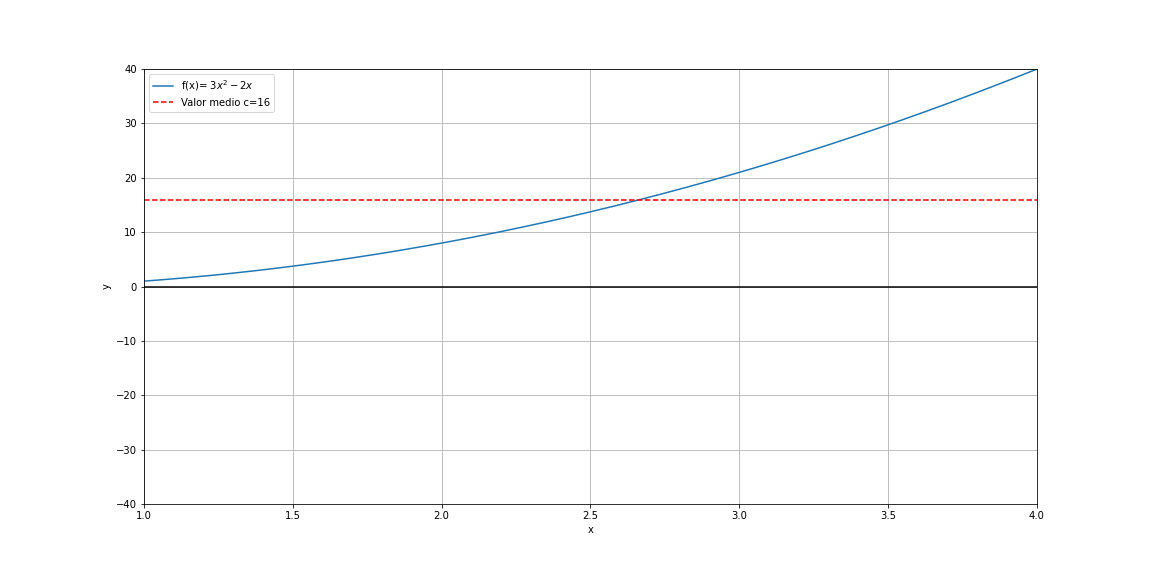
\includegraphics[scale=0.28]{ext3.png}
\caption{Representación gráfica del valor medio de la función.} \label{ext3}
\end{figure}
\end{center}
\end{myexample}

\begin{myexample}
 A un paciente se le inyecta 2 miligramos de un medicamento a la vena. La cantidad de medicamento que se queda en la sangre después de t horas está dado por $f(t)=f_{0}e^{-0,32\cdot t}$, donde $f_{0}$ es la cantidad inicial del medicamento. Encuentre la cantidad promedio de medicamento en la sangre solamente de la segunda hora.\\

\begin{eqnarray*}
f(c)&=&\dfrac{1}{2-1}\int_{1}^{2}2e^{-0,32\cdot t}dt\\
&=& 2\left[\dfrac{e^{-0,32\cdot t}}{-0,32} \right]\\
&=& \dfrac{2}{-0,32}\left[e^{-0,32\cdot t}\right]\Bigg|_{1}^{2}\\
&=& \dfrac{2}{-0,32}\left[e^{-0,32\cdot 2}-e^{-0,32\cdot 1}\right]\\
&=& \dfrac{2\cdot e^{-0,32}}{-0,32}\left[e^{-0,32}-1\right]\\
\end{eqnarray*}
 \end{myexample}
